\let\lesson\undefined
\newcommand{\lesson}{\phantomlesson{Bài 17.}}
\let\lesson\undefined
\newcommand{\lesson}{\phantomlesson{Bài 17.}}


\setcounter{section}{2}
\section{Trắc nghiệm}
\Opensolutionfile{ans}[ans/VN12-Y24-PH-SYL-032P-TN]
\setcounter{ex}{0}
% ===================================================================
\begin{ex}\mkstar{1}
	 Phát biểu nào sau đây là \textbf{sai} khi nói về độ phóng xạ?
	\choice
	{Độ phóng xạ là đại lượng đặc trưng cho tính phóng xạ mạnh hay yếu của một lượng chất phóng xạ}
	{Đơn vị đo độ phóng xạ là becquerel}
	{Với mỗi lượng chất phóng xạ xác định thì độ phóng xạ tỉ lệ với số nguyên tử của lượng chất đó}
	{\True Độ phóng xạ của một lượng chất phóng xạ phụ thuộc nhiệt độ của lượng chất đó}
	\loigiai{}
\end{ex}
% ===================================================================
\begin{ex}\mkstar{2}
	Hình bên dưới là mặt đồng hồ của máy bay thế chiến II phát sáng trong bóng tối, vì chúng được sơn bằng sơn phát quang pha radium (có chu kì bán rã 1602 năm). Mặc dù mặt đồng hồ sơn radium có thể nhìn thấy dễ dàng cả ngày lẫn đêm, nhưng chúng phát ra radon, một loại khí phóng xạ nguy hiểm và không thể cảm nhận trực tiếp. 
	\begin{center}
		\includegraphics[width=0.4\linewidth]{../figs/VN12-Y24-PH-SYL-032P-1}
		\captionof{figure}{Mặt đồng hồ trong máy bay được sơn bằng sơn phát quang có pha radium.}
	\end{center}
	Nếu độ phóng xạ ban đầu của radium khi mới được sơn là $\SI{E5}{\becquerel}$ thì độ phóng xạ còn lại sau 57 năm kể từ khi sản xuất là
	\choice
	{$\SI{96504.5}{\becquerel}$}
	{$\SI{2436.1}{\becquerel}$}
	{\True $\SI{97563.9}{\becquerel}$}
	{$\SI{3495.5}{\becquerel}$}
	\loigiai{
		Độ phóng xạ còn lại:
		$$H=H_0\cdot 2^{-\dfrac{t}{T}}=\left(\SI{E5}{\becquerel}\right)\cdot 2^{-\dfrac{57}{1602}}\approx\SI{97563.9}{\becquerel}.$$
	}
\end{ex}
% ===================================================================
\begin{ex}\mkstar{2}
	Hiện nay đồng vị phóng xạ $\ce{_9^{18}F}$ được sử dụng rộng rãi trong việc chẩn đoán các bệnh ung thư nhờ vào công nghệ chụp cắt lớp bằng phát xạ positron (Positron Emission Tomography - PET). Giả sử rằng một bệnh nhân được tiêm một lượng chất phóng xạ $\ce{_9^{18}F}$ với độ phóng xạ là $\SI{350}{\becquerel}$ trước khi quá trình chụp ảnh diễn ra. Hỏi sau bao lâu kể từ thời điểm tiêm thì độ phóng xạ trong cơ thể bệnh nhân giảm còn $\SI{25}{\becquerel}$? Biết rằng chu kì bán rã của $\ce{_9^{18}F}$ là 110 ngày.
	\choice
	{378,92 ngày}
	{427,93 ngày}
	{\True 418,81 ngày}
	{125,46 ngày}
	\loigiai{
	Khoảng thời gian cần tìm là:
	$$H_t=H_02^{-\dfrac{t}{T}}\Rightarrow 25=350\cdot 2^{-\frac{t}{110}}\Rightarrow t\approx\SI{418.81}{\text{ngày}}.$$
	}
\end{ex}
% ===================================================================
\begin{ex}\mkstar{3}
	Nguồn polonium $\left(\ce{^{210}Po}\right)$ được sử dụng trong phòng thí nghiệm vật lý có độ phóng xạ $\SI{1.0}{\micro Ci}$ vào ngày chuẩn bị mẫu. Sau 120 ngày, một sinh viên vào phòng thí nghiệm đo độ phóng xạ của nguồn bằng máy đếm Geiger và thu được 1500 lần đếm mỗi phút. Biết chu kì bán rã của polonium là 138 ngày. Trong thí nghiệm trên, máy đã ghi nhận được bao nhiêu phần trăm phân rã do nguồn phát ra?
	\choice
	{$\SI{12.3}{\percent}$}
	{$\SI{0.74}{\percent}$}
	{$\SI{7.4}{\percent}$}
	{\True $\SI{0.123}{\percent}$}
	\loigiai{
		Độ phóng xạ còn lại sau 120 ngày:
		$$H=H_0\cdot2^{-\dfrac{t}{T}}=\left(\SI{E-6}{Ci}\right)\cdot\left(\SI{3.7E10}{\becquerel/Ci}\right)\cdot 2^{-\dfrac{120}{138}}=\SI{20250.5}{\becquerel}.$$
		Số phân rã trong 1 phút sau 120 ngày:
		$$\Delta N=H\Delta t=\left(\SI{20250.5}{\becquerel}\right)\cdot\left(\SI{60}{\second}\right)=\SI{1215032}{\text{phân rã}}.$$
		Tỉ lệ phân rã được máy ghi nhận:
		$$\dfrac{\Delta N'}{\Delta N}\cdot\SI{100}{\percent}=\dfrac{1500}{1215032}\cdot\SI{100}{\percent}\approx\SI{0.123}{\percent}.$$
	}
\end{ex}
% ===================================================================
\begin{ex}\mkstar{4}
	Trong khảo cổ học để đánh giá tuổi của các vật liệu hữu cơ như gỗ và da, người ta thường sử dụng kỹ thuật xác định tuổi bằng carbon phóng xạ. Cơ sở của kĩ thuật này là mật độ  nguyên tử $\ce{^{14}C}$ trong khí quyển gần như không đổi và có giá trị bằng $1,3$ nguyên tử $\ce{^{14}C}$ trong mỗi $10^{12}$ nguyên tử carbon bao gồm tất cả các đồng vị. Tuy nhiên, khi một cơ thể sống chết đi, $\ce{^{14}C}$ không còn được cung cấp nữa và bắt đầu giảm đi phóng xạ $\beta$ với thời gian bán rã $\SI{5730}{\text{năm}}$:
	$$\ce{^{14}_6C}\longrightarrow \ce{^{14}_7N}+e^{-}+\overline{\nu}_e$$
	Giả sử có $\SI{50}{\gram}$ carbon từ một mảnh gỗ tìm được trong một ngôi mộ tiền sử. Biết khối lượng nguyên tử trung bình của carbon là $\SI{2e-26}{\kilogram}$. Người ta không thể đếm trực tiếp số nguyên tử $\ce{^{14}C}$ được nhưng có thể đếm được tổng số $935$ electron phát xạ từ mảnh gỗ trên trong 10 phút. Tuổi của ngôi mộ là
	\choice
	{19359 năm}
	{\True 17190 năm}
	{13223 năm}
	{15021 năm}
	\loigiai{
		Số nguyên tử $\ce{^{14}C}$ ban đầu trong mảnh gỗ:
		$$N_0=\dfrac{m}{m_0}\cdot\dfrac{1,3}{10^12}=\SI{3.25E12}{}.$$
		Độ phóng xạ của mẫu gỗ ở thời điểm phát hiện:
		$$H=\dfrac{\Delta N}{\Delta t}=\lambda N_0e^{-\lambda T}$$
		Tuổi của mẫu vật:
		$$\begin{aligned}
			&t=-\dfrac{1}{\lambda}\cdot\ln\left(\dfrac{1}{\lambda N_0}\cdot\dfrac{\Delta N}{\Delta t}\right)=-\dfrac{T}{\ln2}\cdot\ln\left(\dfrac{T}{N_0\ln 2}\cdot\dfrac{\Delta N}{\Delta t}\right)\\
			\Rightarrow &t=-\dfrac{\left(\SI{5730}{\text{năm}}\right)}{\ln2}\cdot\ln\left(\dfrac{5730\cdot365\cdot24\cdot\SI{60}{\minute}}{\SI{3.25E12}{}\cdot\ln2}\cdot\dfrac{935}{\SI{10}{\minute}}\right)\approx\SI{17190}{\text{năm}}.
		\end{aligned}
		$$}
\end{ex}

\Closesolutionfile{ans}
\section{Trắc nghiệm đúng/sai}
\Opensolutionfile{ans}[ans/VN12-Y24-PH-SYL-032P-TF]
\setcounter{ex}{0}
% ===================================================================
\begin{ex}\mkstar{1}
	Nhận định các phát biểu sau:
	\choiceTF[t]
	{Phân rã phóng xạ cần có kích thích để xảy ra}
	{\True Tia phóng xạ là tia không nhìn thấy được, nhưng có các tính chất như: ion hóa, gây ra các hiệu ứng quang điện, phát xạ thứ cấp, làm đen kính ảnh, xuyên thấu lớp vật chất mỏng, phá hủy tế bào, kích thích một số phản ứng hóa học, \dots}
	{Tia phóng xạ $\gamma$ là chùm hạt mang điện dương và có khả năng đâm xuyên rất lớn}
	{\True Nguyên tắc an toàn khi làm việc với nguồn phóng xạ: giữ khoảng cách đủ xa đối với nguồn phóng xạ, cần sử dụng các tấm chắn nguồn phóng xạ đủ tốt và cần giảm thiểu thời gian phơi nhiễm phóng xạ}
	\loigiai{}
\end{ex}
% ===================================================================
\begin{ex}\mkstar{2}
	Radon $\left(\ce{^{222}Rn}\right)$ là khí phóng xạ không màu, không mùi, có chu kì bán rã 3,8 ngày. Radon được tạo thành do sự phân rã của uranium, radium, \dots trong đất và đá. Do sự chênh lệch áp suất, radon dễ dàng đi vào trong nhà thông qua các vết nứt, sàn nhà. 
	\begin{center}
		\includegraphics[width=0.4\linewidth]{../figs/VN12-Y24-PH-SYL-032P-2}
		\captionof{figure}{Radon theo các vết nứt trên sàn vào trong nhà.}
	\end{center}
	Radon là chất gây ung thư phổi chỉ sau thuốc lá. Khi được hít vào phổi, radon tích tụ trong phổi và phóng xạ alpha gây tổn thương các mô phổi. Do đó, Cơ quan Bảo vệ Môi trường Hoa Kỳ (EPA) khuyến cáo rằng bất kỳ nhà hoặc văn phòng nào đo trên mức $\SI{4.0}{\pico Ci/\liter}$ cần phải được khắc phục ngay lập tức.
	
	\choiceTF[t]
	{Nếu áp suất trong nhà cao hơn áp suất trong đất, radon dễ dàng vào trong nhà hơn}
	{\True Phương trình phân rã của radon là $\ce{^{222}_{86}Rn}\longrightarrow \ce{^{218}_{84}Po}+\ce{^4_2He}$}
	{Ở các nước ôn đới, chu kì bán rã của radon dài hơn do nhiệt độ thấp}
	{\True Với mức khuyên cáo của EPA ($\SI{4.0}{\pico Ci/\liter}$), một căn nhà kích thước $\SI{5}{\meter}\times \SI{10}{\meter}\times \SI{4}{\meter}$ sẽ có khoảng 14 tỉ nguyên tử radon trong không khí}
	\loigiai{
		\begin{itemchoice}
			\itemch Sai. Nếu áp suất trong nhà thấp hơn áp suất trong đất, radon dễ dàng vào nhà hơn.
			\itemch Đúng. Phương trình thoả bảo toàn số khối và bảo toàn điện tích.
			\itemch Sai. Quá trình phóng xạ không phụ thuộc điều kiện bên ngoài.
			\itemch Đúng. Với độ phóng xạ $h=\SI{4.0}{\pico Ci/\liter}$ thì khối lượng radon trong căn phòng là
			$$\begin{aligned}
				&N=\dfrac{H}{\lambda}=\dfrac{hV}{\lambda}\\
				\Rightarrow & N=\dfrac{\left(\SI{4.0E-9}{Ci/\meter^3}\right)\cdot\left(\SI{3.7E10}{\becquerel/Ci}\right)\cdot\left(\SI{200}{\meter^3}\right)}{\dfrac{\ln 2}{3,8\cdot 24\cdot\SI{3600}{\second}}}\approx\SI{14E9}{\text{hạt}}.
			\end{aligned}$$
		\end{itemchoice}
	}
\end{ex}
% ===================================================================
\begin{ex}\mkstar{3}
	Hai mẫu chất phóng xạ X và Y với chu kì bán rã có đồ thị biểu diễn số hạt phụ thuộc theo thời gian như hình bên. Nhận định các phát biểu sau đây:
	\begin{center}
		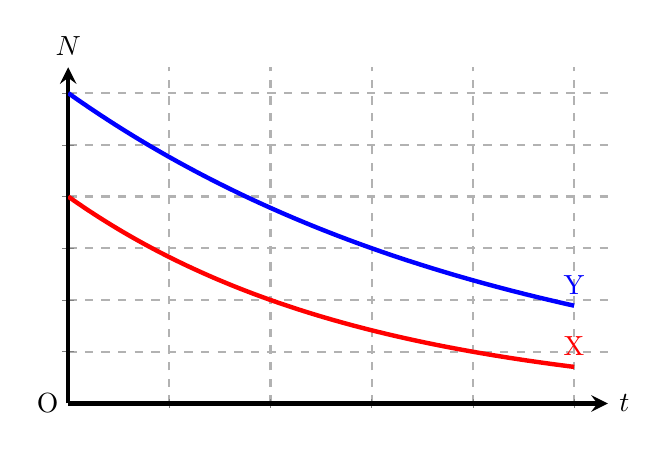
\begin{tikzpicture}  
			\begin{axis}[  ultra thick,yscale=0.75,
				xmin=0,  
				xmax=16,  
				xtick={0,3,...,15},
				ytick={0,1,...,6},
				yticklabels=\empty,
				xticklabels=\empty,
				minor x tick num=0,
				minor y tick num=0,
				ymin=0,  
				ymax=6.5, 
				samples=300,
				axis lines=middle, 
				grid style={step=1, line width =0.4pt, color=gray!30!white},
				grid=both,
				major grid style={line width=0.8pt,gray!60!white, dashed},
				xlabel=$t$, 		ylabel=$N$,
				every axis y label/.style={at=(current axis.above origin),anchor=south},  
				every axis x label/.style={at=(current axis.right of origin),anchor=west},  ]
				\addplot [ultra thick, red, smooth, domain=0:15] {4*2^(-x/6)} node [above] {X};  
				\addplot [ultra thick, blue, smooth, domain=0:15] {6*2^(-x/9)} node [above] {Y};
			\end{axis}  
			\node[left] at (0,0) {O};
		\end{tikzpicture}
		
	\end{center}	
	\choiceTF[t]
	{\True Chu kì bán rã của mẫu Y lớn hơn chu kì bán rã của mẫu X}
	{\True Ban đầu, độ phóng xạ của hai mẫu chất bằng nhau}
	{Tại thời điểm $t=1,75T_{\mathrm{X}}$ (với $T_{\mathrm{X}}$ là chu kì bán rã của mẫu X), hai mẫu chất có số hạt bằng nhau}
	{\True Hằng số phóng xạ của mẫu X gấp 1,5 lần hằng số phóng xạ của mẫu Y}
	\loigiai{
		\begin{itemchoice}
			\itemch Đúng. $T_Y=1,5T_X$.
			\itemch Đúng. Từ độ thị có $N_{0Y}=1,5N_{0X}$ nên
			$$\dfrac{H_{0X}}{H_{0Y}}=\dfrac{N_{0X}}{N_{0Y}}\cdot\dfrac{T_Y}{T_X}=1,5\cdot\dfrac{1}{1,5}=1.$$
			\itemch Sai. Hai mẫu không thể đạt trạng thái có số hạt bằng nhau.
			\itemch Đúng. $\dfrac{\lambda_X}{\lambda_Y}=\dfrac{T_Y}{T_X}=1,5.$
		\end{itemchoice}	
	}
\end{ex}
\Closesolutionfile{ans}
\section{Tự luận}
\Opensolutionfile{ans}[ans/VN12-Y24-PH-SYL-032P-TL]
\setcounter{ex}{0}
% ======================================================================
\begin{ex}\mkstar{2}
	Đồng vị phóng xạ chromium $\ce{_{24}^{51}Cr}$ được sử dụng trong phương pháp nguyên tử đánh dấu của y học hạt nhân khi chẩn đoán các bệnh về thận và huyết học. Chu kì bán rã của chromium $\ce{_{24}^{51}Cr}$ là 27,7 ngày. Mẫu chromium $\ce{_{24}^{51}Cr}$ nguyên chất với độ phóng xạ $\SI{23.9E11}{\becquerel}$ có khối lượng bao nhiêu $\si{\milli\gram}$ \textit{((kết quả làm tròn đến chữ số hàng phần trăm))}?
	\loigiai{$\SI{0.70}{\milli\gram}$}
\end{ex}
% ======================================================================
\begin{ex}\mkstar{2}
	Trong việc điều trị bệnh ung thư bằng phương pháp xạ trị hiện nay, người ta thường sử dụng máy gia tốc hạt trong việc tạo ra các hạt mang năng lượng cao để bắn phá các tế bào ung thư. Tuy nhiên, trước khi máy gia tốc hạt ra đời thì việc điều trị ung thư trong các bệnh viện trước đây lại sử dụng một nguồn phát ra tia gamma như đồng vị phóng xạ $\ce{_{27}{ }^{67}Co}$ (có chu kì bán rã là 5,27 năm, mỗi năm xem như có 365 ngày). Các tia gamma phát ra từ quá trình phóng xạ của $\ce{_{27}^{60}Co}$ được sử dụng để tiêu diệt tế bào ung thư. Hãy tính số lượng hạt nhân $\ce{_{27}^{60}Co}$ chứa trong một nguồn phóng xạ có hoạt độ phóng xạ là $\SI{5800}{ci}$ tại bệnh viện.
	\loigiai{
		Số lượng hạt nhân $\ce{_{27}^{60}Co}$ chứa trong nguồn phóng xạ tại thời điểm đang xét là:
		$$
		H_{t}=\lambda N_{t}=\frac{\ln 2}{T} N_{t}
		$$
		$$\Rightarrow N_{t}=\frac{T}{\ln 2} H_{t}=\frac{5,27 \cdot 365 \cdot 24 \cdot 3600}{\ln 2} \cdot\left(5800 \cdot 3,7 \cdot 10^{10}\right) \approx \SI{5.15E22}{\text{hạt}}$$
	}
\end{ex}
% ======================================================================
\begin{ex}\mkstar{2}
	Để điều trị ung thư tuyến giáp, một bệnh nhân đã nhận một liều dược chất phóng xạ chứa $\SI{25}{\milli\gram}\  \ce{_{53}^{131}I}$. Biết rằng $\ce{_{53}^{131}I}$ là chất phóng xạ $\beta^{-}$ có chu kì bán rã là 8,02 ngày.
	\begin{enumerate}[label=\alph*)]
		\item Viết phương trình phóng xạ của $\ce{_{53}^{131}I}$.
		\item Tính độ phóng xạ của liều thuốc tại thời điểm bệnh nhân sử dụng.
		\item Tính độ phóng xạ của liều thuốc sau khi sử dụng 7,00 ngày.
		\item Tính số hạt $\beta^{-}$phát ra từ liều thuốc trong 7,00 ngày đó.
	\end{enumerate}
	\loigiai{
	\begin{enumerate}[label=\alph*)]
		\item $\ce{^{131}_{53}I}\longrightarrow\ce{^{131}_{54}Xe}+\ce{^0_{-1}e}+\ce{^0_0\bar{v}}$.
		\item $H_0=\SI{1.15E14}{\becquerel}$.
		\item $H=\SI{6.28E13}{\becquerel}$.
		\item $\Delta N=\SI{5.21E19}{\text{electron}}$.
	\end{enumerate}
	}
\end{ex}
	% ===============================================================
\begin{ex}\mkstar{3}
	Một toà nhà vô tình bị nhiễm chất phóng xạ. Trong đó, chất phóng xạ tồn tại lâu nhất là strontium-90 $\left(\ce{^{90}_{38}Sr}\right)$, có khối lượng nguyên tử là $\SI{89.9077}{u}$ và chu kì bán rã 29 năm. Nếu ban đầu trong toà nhà có chứa $\SI{5}{\kilogram}$ chất này và độ an toàn phóng xạ là $\SI{10.0}{\text{phân rã}/\minute}$ thì sau bao lâu toà nhà sẽ trở nên an toàn (kết quả tính theo đơn vị năm và chỉ lấy phần nguyên)?
	\loigiai{
		$$H=\lambda N_0\cdot2^{-\dfrac{t}{T}}=\dfrac{\ln 2}{T}\cdot \dfrac{m}{M}\cdot 2^{-\dfrac{t}{T}}	.$$
		Thời gian để toà nhà  an toàn:
		$$
		\begin{aligned}
			t	&=-T\cdot\log_2\dfrac{HTM}{m\ln 2}=\\
			&=-\left(\SI{29}{\text{năm}}\right)\log_2\dfrac{\left(\xsi{10/60}{\text{phân rã}/\second}\right)\cdot\left(29\cdot365\cdot24\cdot\SI{3600}{\second}\right)\cdot\left(89,9077\cdot\SI{1.6605E-27}{\kilogram}\right)}{\left(\SI{5}{\kilogram}\right)\ln2}\\
			&=\SI{1655}{\text{năm}}.
		\end{aligned}
		$$
		
		
	}
\end{ex}
% ======================================================================
\begin{ex}\mkstar{3}
Các nhà khoa học đã xác định được độ phóng xạ của $\SI{1}{\gram}$ mẫu carbon trong cơ thể sinh vật sống là $\SI{0.231}{\becquerel}$. Biết rằng, trong số các đồng vị của carbon có trong mẫu, chỉ có $\ce{_6^{14}C}$ là đồng vị phóng xạ với chu kì bán rã là 5730 năm.	
\begin{enumerate}[label=\alph*)]
	\item Xác định số nguyên tử $\ce{_6^{14}C}$ có trong $\SI{1}{\gram}$ mẫu carbon đó.
	\item Vào ngày 19/9/1991, trong khi đang tìm đường vượt qua dãy Otztal Alps, hai nhà leo núi người Đức đã phát hiện thấy xác ướp người cổ được bảo quản hầu như nguyên vẹn trong băng tuyết tại Hauslabjoch, khu vực giữa biên giới Áo và Italia. Xác ướp đó được đặt tên là người băng Otzi. Tại thời điểm này, các nhà khoa học đã đo được độ phóng xạ của $
	\SI{1}{\gram}$ mẫu carbon trong cơ thể người băng Otzi là $\SI{0.121}{\becquerel}$. Xác định niên đại của người băng đó.
\end{enumerate}
	\loigiai{
	\begin{enumerate}[label=\alph*)]
		\item $N_0=\SI{6.02E10}{\text{nguyên tử}}$.
		\item $t=\SI{5.35E3}{\text{năm}}$.
	\end{enumerate}
	}
\end{ex}
	% ===============================================================
\begin{ex}\mkstar{3}
	Sự cố hạt nhân diễn ra vào ngày 25 tháng 4 năm 1986 tại nhà máy điện hạt nhân Chernobyl ở Pripyat, Cộng hòa Xã hội chủ nghĩa Xô viết Ukraina được coi là thảm họa hạt nhân tồi tệ nhất trong lịch sử. Do không có tường chắn, lượng lớn phóng xạ từ nhà máy lan rộng ra nhiều vùng phía tây Liên bang Xô viết, Đông Âu và Tây Âu, Scandinavia, Anh quốc, và đông Hoa Kỳ. Người ta ước tính rằng thảm họa Chernobyl đã giải phóng khoảng $\SI{6.0}{\mega Ci} \ce{^{137}Cs}$ vào môi trường. Em hãy xác định khối lượng $\ce{^{137}Cs}$ bị giải phóng (kết quả tính theo đơn vị kilogram và làm tròn đến 1 chữ số thập phân). Biết rằng $\ce{^{137}Cs}$ có chu kì bán rã 30,2 năm. Cho:	
	\begin{itemize}
		\item $\SI{1}{Ci}=\SI{3.7E10}{\becquerel}$;
		\item 1 năm $\approx\SI{3.16E7}{\second}$;
		\item số Avogadro $N_A=\SI{6.022E23}{\mole^{-1}}$.
	\end{itemize}
	\begin{center}
		\begin{tabular}{C{6cm}C{6cm}}
			\includegraphics[width=0.8\linewidth]{../figs/VN12-Y24-PH-SYL-032P-3}
			& \includegraphics[width=0.4\linewidth]{../figs/VN12-Y24-PH-SYL-032P-4}\\
			Nhà máy điện hạt nhân Chernobyl vài tuần sau thảm hoạ & Người phụ nữ cầm con lợn bị dị tật do ảnh hưởng từ bụi phóng xạ.
		\end{tabular}
		
	\end{center}
	\loigiai{
		Từ công thức tính độ phóng xạ:
		$$H=\lambda N=\dfrac{\ln 2}{T}\cdot N$$
		Suy ra, số hạt nhân $\ce{^{137}Cs}$ bị giải phóng ra môi trường khi đó:
		$$N=\dfrac{H\cdot T}{\ln 2}$$
		Khối lượng $\ce{^{137}Cs}$ đã giải phóng vào môi trường:
		$$\begin{aligned}
			m&=\dfrac{N}{N_A}\cdot M=\dfrac{1}{\ln 2}\cdot\dfrac{H\cdot T\cdot M}{N_A}\\
			&=\dfrac{\left(\SI{6.0e6}{Ci}\right)\cdot\left(\SI{3.7E10}{\becquerel/Ci}\right)\cdot\left(\SI{30.2}{\text{năm}}\right)\cdot\left(\SI{3.16E7}{\second/\text{năm}}\right)\cdot\left(\SI{137}{\gram/\mole}\right)}{\ln 2\cdot\left(\SI{6.022E23}{\mole^{-1}}\right)}\approx\SI{69.53E3}{\gram}=\SI{69.53}{\kilogram}.
		\end{aligned}$$
		
	}
\end{ex}
	% ===============================================================
\begin{ex}\mkstar{3}
	Sau tai nạn hạt nhân xảy ra ở lò phản ứng hạt nhân Chernobyl năm 1986, độ phóng xạ trong sữa ở Ba Lan tăng lên $\SI{2000}{\becquerel/\liter}$ do iodine-131, với chu kì bán rã $\SI{8.04}{\text{ngày}}$. Iodine phóng xạ rất nguy hiểm vì tuyến giáp là nơi tích tụ nhiều iodine. Sau sự cố Chernobyl, bệnh ung thư tuyến giáp ở trẻ em Belarus tăng lên đáng kể. Bình thường, trong 1 lít sữa vẫn có chứa $\SI{2.00}{\gram}$ potassium với khoảng $\SI{0.0117}{\percent}$ potassium phóng xạ $\ce{^{40}K}$ có chu kì bán rã $\SI{1.28E9}{\text{năm}}$. Sau bao lâu thì độ phóng xạ do iodine gây ra giảm dưới mức phóng xạ của $\ce{^{40}K}$? Kết quả tính theo đơn vị năm và làm tròn đến 1 chữ số thập phân.
	\loigiai{
		Độ phóng xạ của $\ce{^{40}K}$ trong sữa bình thường:
		$$H=\lambda_{\ce{K}}\cdot\dfrac{m_{\ce{^{40}K}}}{M_{\ce{^40}K}}\cdot N_A=\dfrac{\ln 2}{\left(\SI{1.28E9}{}\cdot365\cdot24\cdot\SI{3600}{\second}\right)}\cdot\dfrac{\left(\SI{0.0117}{\percent}\right)\cdot\SI{2}{\gram}}{\SI{40}{\gram/\mole}}\cdot\left(\SI{6.022E23}{\mole^{-1}}\right)=\SI{60.49}{\becquerel}.$$		
		Thời gian để độ phóng xạ iodine giảm dưới mức phóng xạ của $\ce{^{40}K}$ trong sữa bình thường:
		$$H=H_02^{-\dfrac{t}{T_{\ce{I}}}}\Rightarrow t=-T_{\ce{I}}\cdot\log_2\left(\dfrac{H}{H_0}\right)\approx\SI{40.6}{\text{năm}}.$$
		
		
	}
\end{ex}
% ======================================================================
\begin{ex}\mkstar{3}
	Để xác định lượng máu trong bệnh nhân, người ta tiêm vào máu một người một lượng nhỏ dung dịch chứa đồng vị phóng xậ $\ce{^{24}Na}$ (chu kì bán rã 15 giờ) có độ phóng xạ $\SI{2}{\micro ci}$. Sau 7,5 giờ người ta lấy ra $\SI{1}{\centi\meter^3}$ máu người đó thì thấy có độ phóng xạ 502 phân rã/phút. Tính thể tích máu của người đó.	
	\loigiai{
		Đổi $\ce{H}_0=\SI{2}{\micro ci}=2 \cdot 10^{-6} \cdot 3,7 \cdot 10^{10}=\SI{7.4E4}{\becquerel}$; $\ce{H}=\xsi{502V}{\text{phân rã/phút}}$ ($V$ là thể tích của máu: $\si{\centi\meter^3}$)
		$$
		\begin{aligned}
			& \ce{H}=\ce{H}_0 2^{-\frac{\ce{t}}{\ce{T}}}=\ce{H}_0 2^{-0,5} \Rightarrow \frac{\ce{H}}{\ce{H}_0}=2^{-0,5}=\frac{8,37V}{7,4 \cdot 10^4} \Rightarrow 8,37V=7,4 \cdot 10^4 \cdot 2^{-0,5} \\
			& \Rightarrow V=\frac{7,4 \cdot 10^4 \cdot 2^{-0,5}}{8,37}=\SI{6251.6}{\centi\meter^3}=\SI{6.25}{\deci\meter^3}=\SI{6.25}{\liter}.
		\end{aligned}
		$$
	}
\end{ex}
% ======================================================================
\begin{ex}\mkstar{4}
	Hiện nay, một trong những phương pháp xác định tuổi của một mẫu vật cổ thông dụng được các nhà địa chất và khảo cổ học sử dụng chính là dựa vào việc đo hoạt độ phóng xạ của đồng vị $\ce{_6^{14}C}$. Trong bài tập này, chúng ta sẽ lần lượt nghiên cứu sự hình thành $\ce{_6^{14}C}$ và ứng dụng của nó thông qua các câu hỏi dưới đây:
	\begin{enumerate}[label=\alph*)]
		\item Sự tạo thành $\ce{_6^{14}C}$: Neutron năng lượng cao trong các tia vũ trụ trước khi đến bề mặt Trái Đất sẽ đi qua bầu khí quyển. Tại đó, chúng phản ứng với các hạt nhân $\ce{_7^{14}N}$ (theo tỉ lệ $1:1$ ) và tạo thành $\ce{_6^{14}C}$ cùng với hạt nhân $X$. Viết phương trình phản ứng xảy ra và xác định $X$.
		\item Trong quá trình tiếp theo, cứ một nguyên tử carbon được tạo thành kết hợp với hai nguyên tử oxygen trong bầu khí quyển để tạo thành một phân tử $\ce{CO_2}$. Các sinh vật trên Trái Đất hấp thụ đồng vị $\ce{_6^{14}C}$ thông qua quá trình quang hợp, tiêu thụ thức ăn, \dots làm cho hàm lượng $\ce{_6^{14}C}$ duy trì ổn định. Tuy nhiên, khi sinh vật chết đi, vì không còn nguồn cung nữa nên hàm lượng $\ce{_6^{14}C}$ trong sinh vật đó sẽ giảm xuống do phân rã $\beta$ với chu kì bán rã là 5730 năm.\\ 
		Em hãy viết phương trình phân rã của $\ce{_6^{14}C}$.
		\item Xét một mảnh gỗ hoá thạch có khối lượng carbon chứa trong đó là $\SI{220}{\gram}$. Tại thời điểm nghiên cứu, người ta đo được hoạt độ phóng xạ của mảnh gỗ này là $\SI{0.52}{\becquerel}$. Hãy xác định tuổi của mẫu gỗ hoá thạch nói trên. Biết rằng trong gỗ đang sống, tỉ số nguyên tử giữa hai đồng vị $\ce{_6^{14}C}$ và $\ce{_6^{12}C}$ (bền) là $\SI{1.3E-12}{}$. Lấy gần đúng khối lượng của hạt nhân bằng số khối của nó và số Avogadro là $N_{A} \approx \SI{6.022E23}{\mole^{-1}}$.
	\end{enumerate}
	\loigiai{
		\begin{enumerate}[label=\alph*)]
			\item $\ce{_0^1n}+{ }_7^{14} \ce{N} \longrightarrow\ce{_6^{14}C}+ \ce{_1^1p}$. Vậy $\ce{X}$ chính là hạt proton.
			\item $\ce{_6^{14}C} \longrightarrow\ce{_7^{14}N}+\ce{_{-1}^0e}+\bar{v}_{\ce{e}}$.
			\item Số lượng hạt nhân $\ce{_6^{14}C}$ trong mảnh gỗ hiện tại là:
			$$
			N_{\ce{C} 14}=\frac{H}{\lambda}=\frac{T}{\ln 2} H
			$$
			Khối lượng $\ce{_6^{14}C}$ trong mảnh gỗ hiện tại là:
			$$
			m_{\ce{C} 14}=\frac{N_{\ce{C} 14}}{N_{A}} \cdot A_{\ce{C} 14}=\frac{T}{\ln 2} \cdot \frac{A_{\ce{C} 14}}{N_{A}} \cdot H
			$$
			Số lượng hạt nhân $\ce{_6^{12}C}$ trong mảnh gỗ hiện tại là:
			$$
			N_{\ce{C} 12}=\frac{m_{\ce{C} 12}}{A_{\ce{Cl} 2}} \cdot N_{A}=\frac{m-m_{\ce{C} 14}}{A_{\ce{Cl} 2}} \cdot N_{A}=\frac{m}{A_{\ce{C} 12}} \cdot N_{A}-\frac{T}{\ln 2} \cdot \frac{A_{\ce{C} 14}}{A_{\ce{Cl} 2}} \cdot H
			$$
			Vì đồng vị $\ce{_6^{12}C}$ bền nên số lượng hạt nhân $\ce{_6^{12}C}$ được xem gần đúng là không đổi. Từ đó ta suy ra số lượng hạt nhân $\ce{_6^{14}C}$ tại thời điểm ban đầu (lúc khối gỗ còn đang sống) là:
			$$
			N_{0(\ce{C}14)}=1,3 \cdot 10^{-12} \cdot N_{\ce{C}12}
			$$
			Độ tuổi của mẫu hoá thạch là:
			$$
			\begin{aligned}
				& N_{\ce{C} 14}=N_{0\left(\ce{C14}\right)} 2^{-\frac{t}{T}} \\
				& \Rightarrow t=-T \log _2\left(\frac{N_{\ce{C} 14}}{N_{0(\ce{C} 14)}}\right)=-5730 \cdot \log_2\left[\frac{T}{1,3 \cdot 10^{-12}} \cdot \frac{H A_{\ce{C} 12}}{\left(m N_A \ln 2-A_{\ce{C} 14} H T\right)}\right] \\
				&=-5730 \cdot \log _2\left[\frac{5730 \cdot 365 \cdot 24 \cdot 3600 \cdot 0,52 \cdot 12}{1,3 \cdot 10^{-12} \cdot\left[220 \cdot 6,022 \cdot 10^{23} \cdot \ln 2-14 \cdot 0,52 \cdot(5730 \cdot 365 \cdot 24 \cdot 3600)\right]}\right] \\
				& \approx \SI{38541}{\text{năm}}.
			\end{aligned}
			$$
		\end{enumerate}
	}
\end{ex}
\Closesolutionfile{ans}
